\documentclass{article}
\usepackage{amsmath}
\usepackage{graphicx}
\bibliographystyle{IEEEtran}
\usepackage{caption}
\usepackage{subcaption}
%\usepackage{geometry}
\usepackage[colorlinks=true]{hyperref}
\title{Supplemental material for `Eliminating object prior-bias from sparse-projection
tomographic reconstructions'}
\begin{document}
\maketitle
%This supplementary material consists of details of the optimization routine used in our method, links to view our 3D reconstructions and results of 2D reconstructions for different projection views.

\tableofcontents
\newpage
%--------------------------------------------------------------------------
\section{An alternate method to compute weights-map}
The value of $k$ (discussed in Sec.10(C) of the main paper) is typically dependent on the number of false positives the system can allow in exchange for the detection of more true positives (regions of new changes). It is this choice and not the particular type of dataset that affects the selection of $k$. In our work, the chosen $k$ corresponds to the one that gives minimal tolerance to false positives.\\

However, in case one wishes to completely avoid the use of this hyper-parameter, one can construct a binary weights-map using an alternate method described below.

\begin{enumerate}
\item For the purposes of training, treat one of the previously scanned images as test.
\item Annotate the region of differences between the test and all of the previously scanned images based on domain knowledge.
\item Compute the difference between the pilot reconstruction of the test and its projection onto the eigenspace. Let this spatial map be called `error map'.
\item Train a Support Vector Machine (SVM) model to classify patches of this error-map image into one of the two categories: new changes present, new changes absent.
\item Once the trained SVM model is obtained, it can be applied to generate binary weights-map for new test images in the same longitudinal study.
\item Once the binary weights-map $\boldsymbol{W_b}$ is obtained, the prior and the pilot can be stitched by $\boldsymbol{R} = \boldsymbol{W_b}(\rm{Pilot}) + (1-\boldsymbol{W_b})(\rm{Prior})$. Fig.~\ref{fig:okra_svm} shows results of this method on 2D okra dataset.

  Alternatively, these binary weights can also be used in the optimization loop in Eq.~\ref{Eq:main} (corresponding to Eq.~6 in the main paper), although this approach has not been pursued here. 

\begin{equation}
%   \setlength{\belowdisplayskip}{0pt} \setlength{\belowdisplayshortskip}{0pt}
%\setlength{\abovedisplayskip}{-2pt} \setlength{\abovedisplayshortskip}{-2pt}
J_3(\boldsymbol{\theta},\boldsymbol{\alpha}) = \lVert\boldsymbol{\mathcal{R} x}-\boldsymbol{y}\rVert_2^2  + \lambda_1\lVert\boldsymbol{\theta}\rVert_1 +\lambda_2\lVert\boldsymbol{W_b}(\boldsymbol{x} - (\boldsymbol{\mu} + \sum_{k}\boldsymbol{V_k}\alpha_k))\rVert_2^2.
\label{Eq:main}
\end{equation}

\end{enumerate} 

\begin{figure}[!h]
    \begin{subfigure}[b]{0.31\linewidth}
        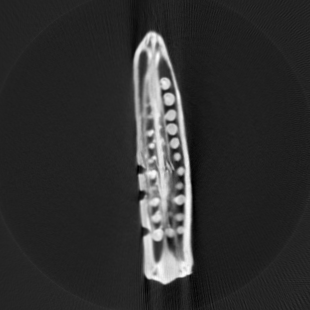
\includegraphics[width=\textwidth]{../images/svm/okra/template_1.png}

        \caption{}
     \end{subfigure}
    \begin{subfigure}[b]{0.31\linewidth}
        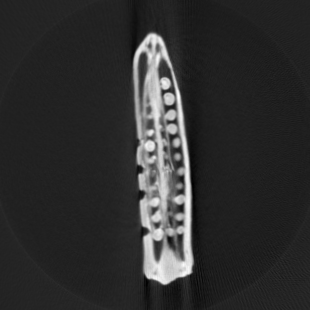
\includegraphics[width=\textwidth]{../images/svm/okra/template_2.png}

        \caption{}
     \end{subfigure}
    \begin{subfigure}[b]{0.31\linewidth}
        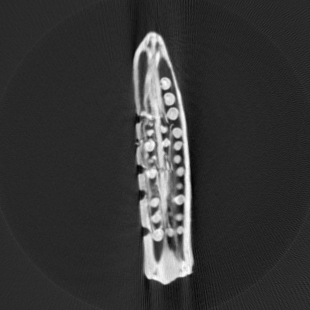
\includegraphics[width=\textwidth]{../images/svm/okra/template_3.png}

        \caption{}
     \end{subfigure}
     \begin{subfigure}[b]{0.31\linewidth}
        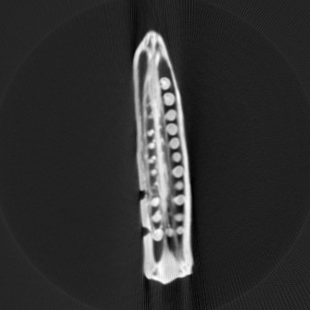
\includegraphics[width=\textwidth]{../images/svm/okra/testIm.png}

        \caption{}
     \end{subfigure}
    \begin{subfigure}[b]{0.31\linewidth}
        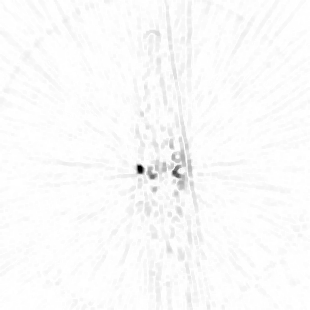
\includegraphics[width=\textwidth]{../images/svm/okra/weights.png}

        \caption{}
     \end{subfigure}
    \begin{subfigure}[b]{0.31\linewidth}
        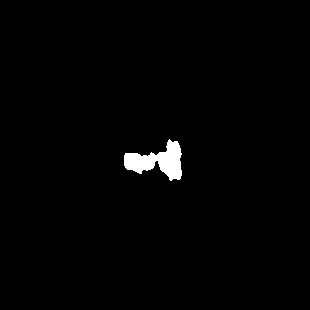
\includegraphics[width=\textwidth]{../images/svm/okra/detectedInlier.png}

        \caption{}
    \end{subfigure}    
    \begin{subfigure}[b]{0.31\linewidth}
        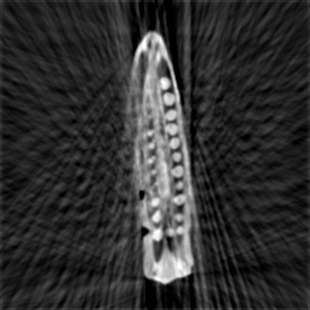
\includegraphics[width=\textwidth]{../images/svm/okra/result_pilot.png}

        \caption{}
    \end{subfigure}
    \quad
    \begin{subfigure}[b]{0.31\linewidth}
        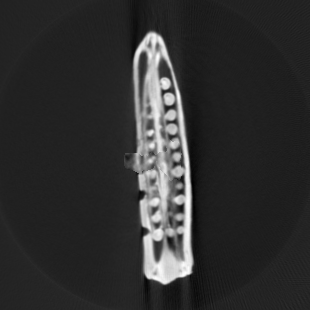
\includegraphics[width=\textwidth]{../images/svm/okra/resultStitched_svm.png}

        \caption{}
     \end{subfigure}
   % \begin{subfigure}[b]{0.19\linewidth}
   %     \includegraphics[width=\textwidth]{images/low_dose_prior/svm_method/prior.png}

    %    \caption{}
    % \end{subfigure}
     \caption[Selecting $k$]{Using an alternate approach to generate (binary) weights map. (a)-(c) the images used as object-prior, (d) the test (310$\times$310). Measurements along $60$ views were taken. (e) error-map showing new regions, (f) detected binary weights map showing regions of new changes, (g) pilot, (h) final reconstruction with pilot in the new regions, and prior in the other regions. } %(h) prior, which is obtained by projecting the pilot onto the eigenspace computed from the templates, 
\label{fig:okra_svm}
\end{figure}
\clearpage
%--------------------------------Links to videos-------------------------------------------------
\newpage
\section{Links to view our 3D reconstructions}
The 3D reconstructions, corresponding to the images shown in Figs.~14,~16 and 19 in the main paper, can be better visualized in the form of a video. Hence, please refer to the following videos to view the 3D datasets and reconstruction results:

\begin{itemize}
\item \textbf{Okra:} \\

  \url{https://www.dropbox.com/sh/x3yjfzsc5633d1t/AAAaVOXvTbc06a2DomPO1kSna?dl=0}\\
\item \textbf{Potato:} \\

  \url{https://www.dropbox.com/sh/6mja5uh8fa2h0fc/AAA2h4VsLxAiXcEIhmTlM1xha?dl=0}\\
\item \textbf{Sprouts:}\\

  \url{https://www.dropbox.com/sh/qtgeyckvbxiaz3s/AADhR2zRUUN4qXSXraErcqSea?dl=0}\\
\end{itemize}

\newpage

%--------------------------BIG images: TMH results
\section{Larger images for reconstruction results}
All the images shown in the main paper are displayed in small size due to space constraints. This restricts visualization of the structural details within them. Therefore, we present each of those images in large size here in order to view their internal structures with better clarity. 
\subsection{Liver}
%-------RFA2 moderate views
%\textbf{Goal: Observe details of new changes}
\begin{figure}[!h]
\centering
\subcaptionbox{Test}{\fcolorbox{white}{blue}{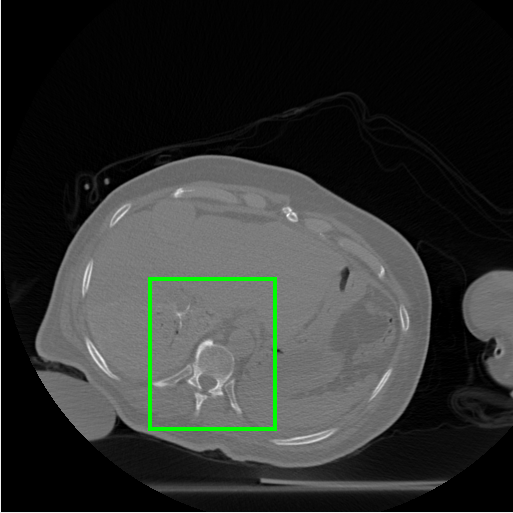
\includegraphics[width=0.49\columnwidth]{../images/tmh/RFA2/few_views/colorTestIm.png}}}\hfill
\subcaptionbox{FBP}{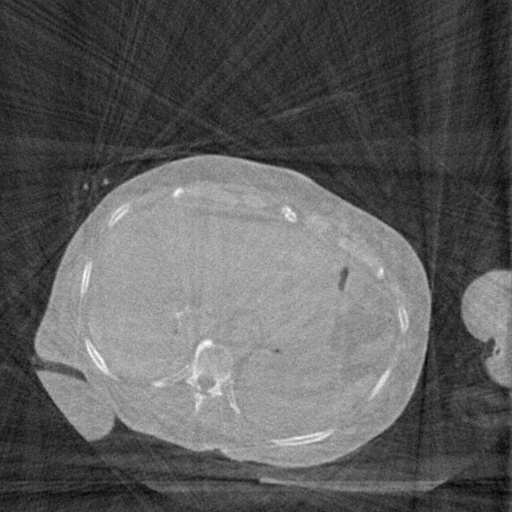
\includegraphics[width=0.49\columnwidth]{../images/tmh/RFA2/few_views/fbp.png}}\hfill
\subcaptionbox{l1-ls}{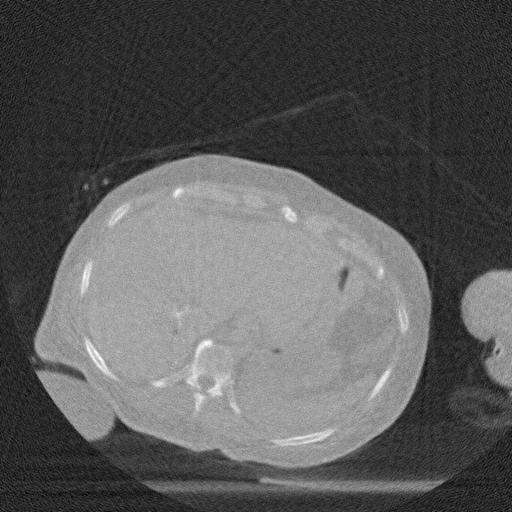
\includegraphics[width=0.49\columnwidth]{../images/tmh/RFA2/few_views/cs_dct.png}}\hfill
\subcaptionbox{Spatially-varying prior}{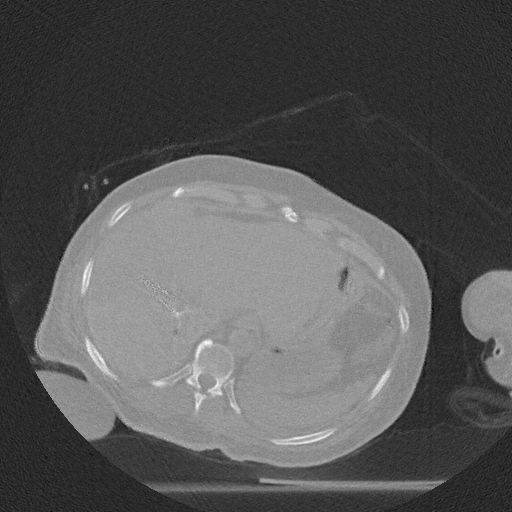
\includegraphics[width=0.49\columnwidth]{../images/tmh/RFA2/few_views/weighted_pca_all_methods_kk_0_01.png}}
\caption[Representative results-2]{Reconstruction of Liver corresponding to Figure 8 of the main paper.}
\label{fig:RFA2_few_views_biggerIm}
\end{figure}
\newpage

\textbf{Test image in Figure~\ref{fig:RFA2_few_views_biggerIm}  is shown in large size for better clarity.}\\
\begin{figure}[!h]
\centering
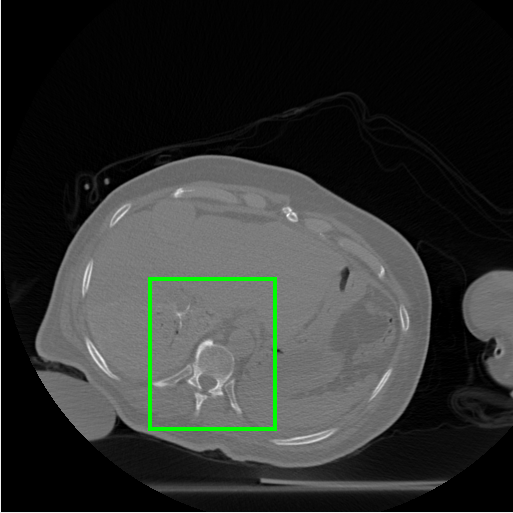
\includegraphics[width=1.2\columnwidth]{../images/tmh/RFA2/few_views/colorTestIm.png}
\captionsetup{labelformat=empty}
\caption[Representative results-2]{\large{Test slice}}
\label{fig:RFA2_few_views_bigger}
\end{figure}
\newpage
\textbf{Reconstruction result of Figure~\ref{fig:RFA2_few_views_biggerIm}   is shown in large size for better clarity.}\\
\begin{figure}[!h]
\centering
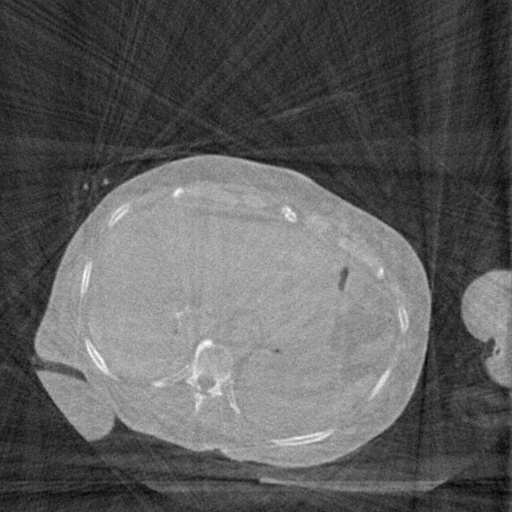
\includegraphics[width=1.2\columnwidth]{../images/tmh/RFA2/few_views/fbp.png}
\captionsetup{labelformat=empty}
\caption[Representative results-2]{\large{FBP}}
\label{fig:RFA2_few_views_bigger}
\end{figure}
\newpage
\textbf{Reconstruction result of Figure~\ref{fig:RFA2_few_views_biggerIm}   is shown in large size for better clarity.}\\
\begin{figure}[!h]
\centering
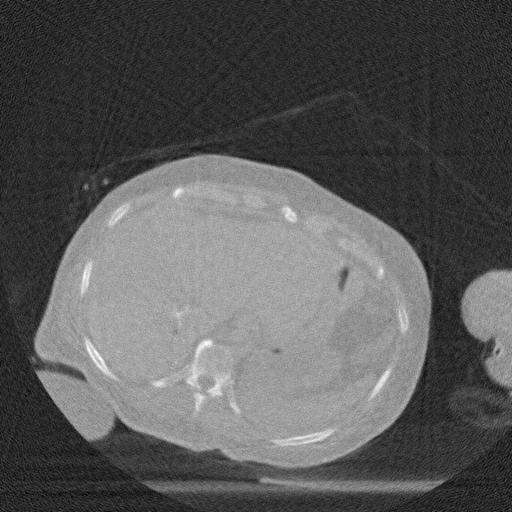
\includegraphics[width=1.2\columnwidth]{../images/tmh/RFA2/few_views/cs_dct.png}
\captionsetup{labelformat=empty}
\caption[Representative results-2]{\large{l1-ls}}
\label{fig:RFA2_few_views_bigger}
\end{figure}
\newpage
\textbf{Reconstruction result of Figure~\ref{fig:RFA2_few_views_biggerIm}  is shown in large size for better clarity.}\\
\begin{figure}[!h]
\centering
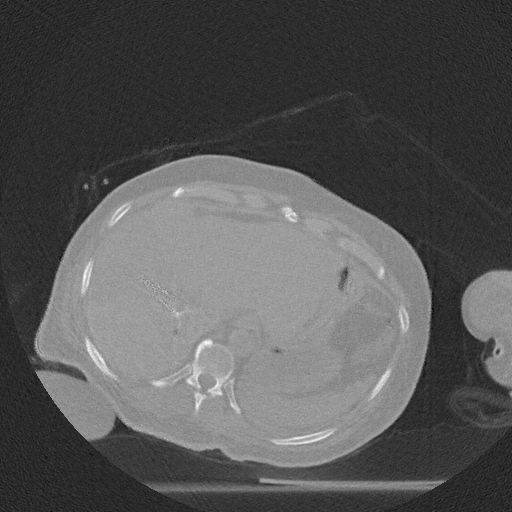
\includegraphics[width=1.2\columnwidth]{../images/tmh/RFA2/few_views/weighted_pca_all_methods_kk_0_01.png}
\captionsetup{labelformat=empty}
\caption[Representative results-2]{\large{Spatially-varying prior method}}
\label{fig:RFA2_few_views_bigger}
\end{figure}
\newpage

%------------------------------------Bigger images for Sprouts------------------
\subsection{Sprouts}
\begin{figure}[!h]
    \begin{subfigure}[b]{0.38\linewidth}
        \fcolorbox{green}{green}{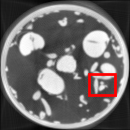
\includegraphics[width=\textwidth]{../images/sprouts/testIm_red.png}}
%\captionsetup{labelformat=empty}
        \caption{Test}
     \end{subfigure}
\quad
    \begin{subfigure}[b]{0.38\linewidth}
        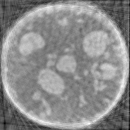
\includegraphics[width=\textwidth]{../images/sprouts/fdkIm.png}
%\captionsetup{labelformat=empty}
        \caption{FDK}
    \end{subfigure}
\quad
    \begin{subfigure}[b]{0.38\linewidth}
        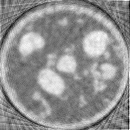
\includegraphics[width=\textwidth]{../images/sprouts/csIm.png}
%\captionsetup{labelformat=empty}
        \caption{l1-ls}
     \end{subfigure}
\quad
    \begin{subfigure}[b]{0.38\linewidth}
        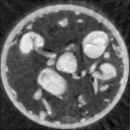
\includegraphics[width=\textwidth]{../images/sprouts/plainPriorIm.png}
%\captionsetup{labelformat=empty}
        \caption{Uniform\\ Prior}
     \end{subfigure}
\quad
    \begin{subfigure}[b]{0.38\linewidth}
        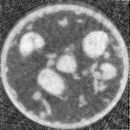
\includegraphics[width=\textwidth]{../images/sprouts/weightedPriorIm.png}
%\captionsetup{labelformat=empty}
        \caption{Spatially-Varying\\ prior}
    \end{subfigure}
    %\quad
    %\captionsetup{labelformat=empty}
     \caption{Reconstruction of sprouts corresponding to Figure 16 of the main paper.} 
\label{fig:sprouts_3D_results_biggerIm}
%\addtolength{\textfloatsep}{-0.8cm}
\end{figure}

\newpage
\textbf{Test image of Figure~\ref{fig:sprouts_3D_results_biggerIm}  is shown in large size for better clarity.}\\
\begin{figure}[!h]
    \begin{subfigure}[b]{\linewidth}
        \fcolorbox{green}{green}{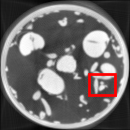
\includegraphics[width=\textwidth]{../images/sprouts/testIm_red.png}}
\captionsetup{labelformat=empty}
        \caption{\large{Test}}
     \end{subfigure}
\end{figure}
\newpage
\textbf{Reconstruction result of Figure~\ref{fig:sprouts_3D_results_biggerIm}  is shown in large size for better clarity.}\\
\begin{figure}[!h]
    \begin{subfigure}[b]{\linewidth}
        \fcolorbox{green}{green}{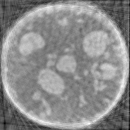
\includegraphics[width=\textwidth]{../images/sprouts/fdkIm.png}}
\captionsetup{labelformat=empty}
        \caption{\large{FDK}}
     \end{subfigure}
\end{figure}
\newpage
\textbf{Reconstruction result of Figure~\ref{fig:sprouts_3D_results_biggerIm}  is shown in large size for better clarity.}\\
\begin{figure}[!h]
    \begin{subfigure}[b]{\linewidth}
        \fcolorbox{green}{green}{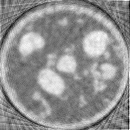
\includegraphics[width=\textwidth]{../images/sprouts/csIm.png}}
\captionsetup{labelformat=empty}
        \caption{\large{l1-ls}}
     \end{subfigure}
\end{figure}
\newpage
\textbf{Reconstruction result of Figure~\ref{fig:sprouts_3D_results_biggerIm}  is shown in large size for better clarity.}\\
\begin{figure}[!h]
    \begin{subfigure}[b]{\linewidth}
        \fcolorbox{green}{green}{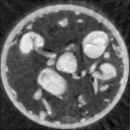
\includegraphics[width=\textwidth]{../images/sprouts/plainPriorIm.png}}
\captionsetup{labelformat=empty}
        \caption{\large{Uniform Prior}}
     \end{subfigure}
\end{figure}
\newpage
\textbf{Reconstruction result of Figure~\ref{fig:sprouts_3D_results_biggerIm}  is shown in large size for better clarity.}\\
\begin{figure}[!h]
    \begin{subfigure}[b]{\linewidth}
        \fcolorbox{green}{green}{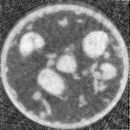
\includegraphics[width=\textwidth]{../images/sprouts/weightedPriorIm.png}}
\captionsetup{labelformat=empty}
        \caption{\large{Spatially-Varying Prior}}
     \end{subfigure}
\end{figure}
\newpage

%--------------------------------Bigger results for Okra------------------------
\subsection{Okra}

\begin{figure}[!h]
\centering
\subcaptionbox{Test}{\fcolorbox{yellow}{yellow}{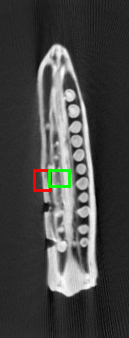
\includegraphics[width=0.2\columnwidth]{../images/okra/testCropped.png}}}\hfill
\subcaptionbox{FDK, no prior}{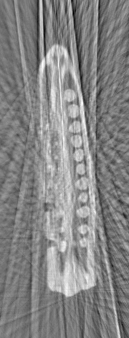
\includegraphics[width=0.2\columnwidth]{../images/okra/fdk_cropped.png}}\hfill
\subcaptionbox{l1-ls}{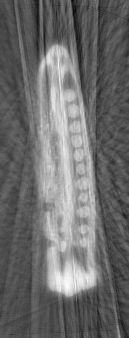
\includegraphics[width=0.2\columnwidth]{../images/okra/cs_cropped.png}}\hfill
\subcaptionbox{\mbox{Uniform}\\prior}{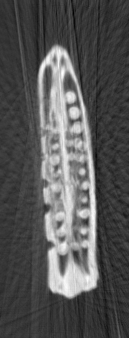
\includegraphics[width=0.2\columnwidth]{../images/okra/pca_cropped.png}}\hfill
\subcaptionbox{Spatially-Varying\\ prior}{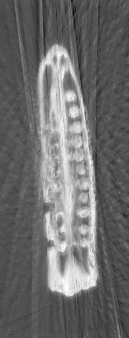
\includegraphics[width=0.2\columnwidth]{../images/okra/prior_weighted_cropped.png}}
\caption{Reconstruction of okra corresponding to Figure 14 of the main paper.}
\label{fig:okra_3D_results_biggerIm}
\end{figure}
\newpage
\textbf{Test image of Figure~\ref{fig:okra_3D_results_biggerIm}   is shown in large size for better clarity.}
\begin{figure}[!h]
\centering
       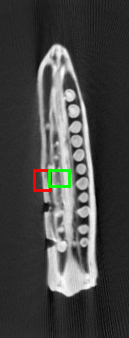
\includegraphics[width=0.5\columnwidth]{../images/okra/testCropped.png}
\captionsetup{labelformat=empty}
        \caption{\large{Test}}
\end{figure}
\newpage

\textbf{Reconstruction result of Figure~\ref{fig:okra_3D_results_biggerIm}  is shown in large size for better clarity.}
\begin{figure}[!h]
\centering
       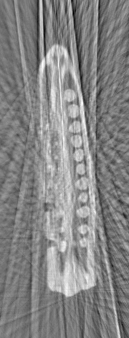
\includegraphics[width=0.5\columnwidth]{../images/okra/fdk_cropped.png}
\captionsetup{labelformat=empty}
        \caption{\large{FDK}}
\end{figure}
\newpage

\textbf{Reconstruction result of Figure~\ref{fig:okra_3D_results_biggerIm}   is shown in large size for better clarity.}
\begin{figure}[!h]
\centering
       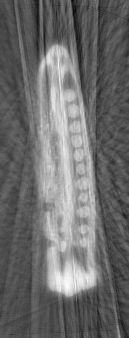
\includegraphics[width=0.5\columnwidth]{../images/okra/cs_cropped.png}
\captionsetup{labelformat=empty}
        \caption{\large{l1-ls}}
\end{figure}
\newpage


\textbf{Reconstruction result of Figure~\ref{fig:okra_3D_results_biggerIm}  is shown in large size for better clarity.}
\begin{figure}[!h]
\centering
       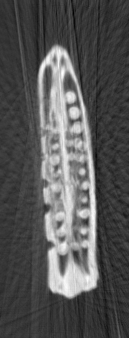
\includegraphics[width=0.5\columnwidth]{../images/okra/pca_cropped.png}
\captionsetup{labelformat=empty}
        \caption{\large{Uniform Prior}}
\end{figure}
\newpage

\textbf{Reconstruction result of Figure~\ref{fig:okra_3D_results_biggerIm}   is shown in large size for better clarity.}
\begin{figure}[!h]
\centering
       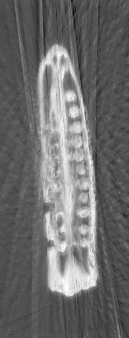
\includegraphics[width=0.5\columnwidth]{../images/okra/prior_weighted_cropped.png}
\captionsetup{labelformat=empty}
        \caption{\large{Spatially-Varying prior}}
\end{figure}
\newpage

%----------------------------------Comparison with Literature------------------------
\section{Detecting new changes directly in the measurements}

Sec.2 of the main paper (`Related work') contrasts the spatially-varying technique  with other prior based techniques in literature. Here we present a 2D reconstruction  result (of the test shown in Figure.~\ref{fig:comparisonLit_dataset}) to compare our method with~\cite{Lee2012}, in which the new changes are directly detected in the measurement space by computing the difference between the measurements of the test and the corresponding simulated measurements of the template. This difference-volume is then reconstructed and then fused (added to) with the original high quality template. However, in the above method, the sub-sampling artefacts present in the difference-volume gets carried over to the final reconstructed image. This is shown in Figure~\ref{fig:comparisonLit_results}. A quantitative comparison over the region of interest is shown in Table~\ref{tab:comparisonLit}.
\begin{figure}[!h]
    \begin{subfigure}[b]{0.4\linewidth}
        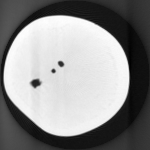
\includegraphics[width=\textwidth]{../images/potato/template_3.png}
%\captionsetup{labelformat=empty}
        \caption{Template}
     \end{subfigure}
\quad
    \begin{subfigure}[b]{0.4\linewidth}
        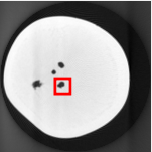
\includegraphics[width=\textwidth]{../images/potato/testIm_color.png}
%\captionsetup{labelformat=empty}
        \caption{Test}
    \end{subfigure}
    %\captionsetup{labelformat=empty}
     \caption{Template and test from the Potato dataset for the reconstructions shown in Figure.~\ref{fig:comparisonLit_results}} 
\label{fig:comparisonLit_dataset}
%\addtolength{\textfloatsep}{-0.8cm}
\end{figure}
\newpage

\begin{figure}[!h]
    \begin{subfigure}[b]{0.4\linewidth}
        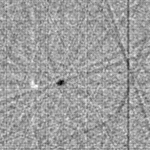
\includegraphics[width=\textwidth]{../images/comparison_lit/result_new_changes.png}
%\captionsetup{labelformat=empty}
        \caption{~\cite{Lee2012}:new-changes}
     \end{subfigure}
\quad
    \begin{subfigure}[b]{0.4\linewidth}
        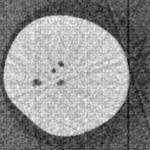
\includegraphics[width=\textwidth]{../images/comparison_lit/result_literature_test.png}
%\captionsetup{labelformat=empty}
        \caption{~\cite{Lee2012}:Reconstruction}
    \end{subfigure}

    \begin{subfigure}[b]{0.4\linewidth}
        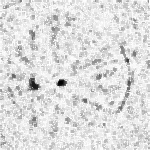
\includegraphics[width=\textwidth]{../images/comparison_lit/weightsIm_all_methods30.png}
%\captionsetup{labelformat=empty}
        \caption{Our weights-map}
    \end{subfigure}
   \quad
        \begin{subfigure}[b]{0.4\linewidth}
        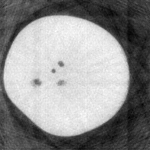
\includegraphics[width=\textwidth]{../images/comparison_lit/weighted_pca_all_methods30.png}
%\captionsetup{labelformat=empty}
        \caption{Our Reconstruction}
    \end{subfigure}
    %\captionsetup{labelformat=empty}
     \caption{Reconstruction of the test in Figure~\ref{fig:comparisonLit_dataset}.  Reconstructions were performed from 12 views. Gaussian noise of 0 mean and SD = $1\%$ of mean of measurements, was added to the measurements.} 
\label{fig:comparisonLit_results}
%\addtolength{\textfloatsep}{-0.8cm}
\end{figure}

\begin{table}[!h]
  \centering
      \caption{SSIM values (within RoI) of reconstructions shown in Figure~\ref{fig:comparisonLit_results}}
  \begin{tabular}{|l|l|l|}
\hline
 & \textbf{SSIM (whole image)} & \textbf{SSIM (RoI)} \\ \hline
\textbf{Method in~\cite{Lee2012}} & 0.65 & 0.60 \\ \hline
\textbf{\begin{tabular}[c]{@{}l@{}}Spatially-varying \\prior\end{tabular}} & 0.89 & 0.92 \\ \hline
  \end{tabular}
  \label{tab:comparisonLit}
\end{table}
\newpage
%-----------------------------------Blurred results (CS)
\section{Blurred reconstruction under limited views}

The l1-ls reconstructions shown in the main paper (for example, in Figs.~14(c),~16(c) and 19(c)), appear to be blurred. Here, we discuss the reason for this observation by reconstructing an image from varying number of views using l1-ls (Eq.1 in the main paper).\\

When the number of views is large, the reconstruction using l1-ls is indeed good, as shown below in Fig~\ref{fig:cs_blurred_48_views}. For the reconstructions shown below, we have tuned the $\lambda_1$ values (Figs.~\ref{fig:ssim_rmse_48_views},~\ref{fig:ssim_rmse_24_views},~\ref{fig:ssim_rmse_12_views}) and selected the one with maximum SSIM. 


\begin{figure}[!h]
    \begin{subfigure}[b]{0.3\linewidth}
        \includegraphics[width=\textwidth]{../images/potato/2D/cs_blurred_results/48_views/testIm.png}
%\captionsetup{labelformat=empty}
        \caption{Test}
     \end{subfigure}
\quad
    \begin{subfigure}[b]{0.3\linewidth}
        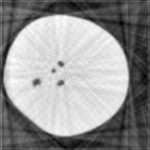
\includegraphics[width=\textwidth]{../images/potato/2D/cs_blurred_results/48_views/result_FBP.png}
%\captionsetup{labelformat=empty}
        \caption{FDK}
    \end{subfigure}
    \begin{subfigure}[b]{0.3\linewidth}
        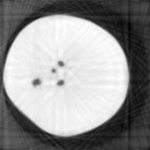
\includegraphics[width=\textwidth]{../images/potato/2D/cs_blurred_results/48_views/result_CS_lambda0_0.40.png}
%\captionsetup{labelformat=empty}
        \caption{l1-ls}
    \end{subfigure}
    %\captionsetup{labelformat=empty}
     \caption{Reconstruction of potato test slice (150$\times$150) from 48 views. The $\lambda_1$ for l1-ls reconstruction was chosen to be the optimal value of 0.4 here.} 
\label{fig:cs_blurred_48_views}
%\addtolength{\textfloatsep}{-0.8cm}
\end{figure}

\begin{figure}[!h]
\centering
       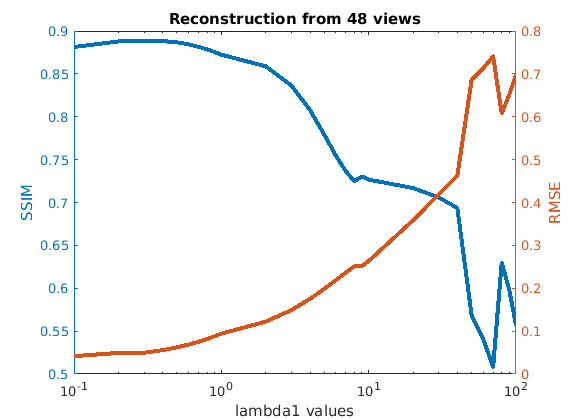
\includegraphics[width=0.9\columnwidth]{../images/potato/2D/cs_blurred_results/SSIM_RMSE_48_angles.png}
%\captionsetup{labelformat=empty}
\caption{SSIM and RMSE for reconstruction from 48 views for varying levels of $\lambda_1$. The optimal value of 0.4 was chosen to obtain the reconstruction shown in Fig.~\ref{fig:cs_blurred_48_views}}
\label{fig:ssim_rmse_48_views}
\end{figure}
\newpage

However, when the number of views decreases, the reconstruction using l1-ls is blurred, but with the benefit of suppressed artefacts that are otherwise present in FBP reconstruction. This is illustrated in Figs.~\ref{fig:cs_blurred_24_views} and~\ref{fig:cs_blurred_12_views}.


\begin{figure}[!h]
    \begin{subfigure}[b]{0.3\linewidth}
        \includegraphics[width=\textwidth]{../images/potato/2D/cs_blurred_results/24_views/testIm.png}
%\captionsetup{labelformat=empty}
        \caption{Test}
     \end{subfigure}
\quad
    \begin{subfigure}[b]{0.3\linewidth}
        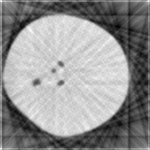
\includegraphics[width=\textwidth]{../images/potato/2D/cs_blurred_results/24_views/result_FBP.png}
%\captionsetup{labelformat=empty}
        \caption{FDK}
    \end{subfigure}
    \begin{subfigure}[b]{0.3\linewidth}
        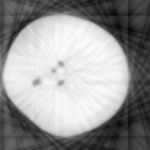
\includegraphics[width=\textwidth]{../images/potato/2D/cs_blurred_results/24_views/result_CS_lambda0_2.00.png}
%\captionsetup{labelformat=empty}
        \caption{l1-ls}
    \end{subfigure}
    %\captionsetup{labelformat=empty}
     \caption{Reconstruction of potato test slice (150$\times$150) from 24 views. The $\lambda_1$ for l1-ls reconstruction was chosen to be the optimal value of 2 here.} 
\label{fig:cs_blurred_24_views}
%\addtolength{\textfloatsep}{-0.8cm}
\end{figure}

\begin{figure}[!h]
\centering
       \includegraphics[width=\columnwidth]{../images/potato/2D/cs_blurred_results/SSIM_RMSE_24_angles.png}
%\captionsetup{labelformat=empty}
\caption{SSIM and RMSE for reconstruction from 24 views for varying levels of $\lambda_1$. The optimal value of 2 was chosen to obtain the reconstruction shown in Fig.~\ref{fig:cs_blurred_24_views}}
\label{fig:ssim_rmse_24_views}
\end{figure}
\newpage

\begin{figure}[!h]
    \begin{subfigure}[b]{0.3\linewidth}
        \includegraphics[width=\textwidth]{../images/potato/2D/cs_blurred_results/12_views/testIm.png}
%\captionsetup{labelformat=empty}
        \caption{Test}
     \end{subfigure}
\quad
    \begin{subfigure}[b]{0.3\linewidth}
        \includegraphics[width=\textwidth]{../images/potato/2D/cs_blurred_results/12_views/result_FBP.png}
%\captionsetup{labelformat=empty}
        \caption{FDK}
    \end{subfigure}
    \begin{subfigure}[b]{0.3\linewidth}
        \includegraphics[width=\textwidth]{../images/potato/2D/cs_blurred_results/12_views/result_CS_lambda0_3.00.png}
%\captionsetup{labelformat=empty}
        \caption{l1-ls}
    \end{subfigure}
    %\captionsetup{labelformat=empty}
     \caption{Reconstruction of potato test slice (150$\times$150) from 12 views. The $\lambda_1$ for l1-ls reconstruction was chosen to be the optimal value of 3 here.} 
\label{fig:cs_blurred_12_views}
%\addtolength{\textfloatsep}{-0.8cm}
\end{figure}
As seen here, the reconstruction by l1-ls is indeed blurred when the number of views is very less. The iterative reconstruction was run until convergence (epsilon = 0.001).
%The plots below show the SSIM and RMSE values for varying values of lambda1 for the CS (LASSO) reconstructions of the above test image.

\begin{figure}[!h]
\centering
       \includegraphics[width=\columnwidth]{../images/potato/2D/cs_blurred_results/SSIM_RMSE_12_angles.png}
%\captionsetup{labelformat=empty}
\caption{SSIM and RMSE for reconstruction from 12 views for varying levels of $\lambda_1$. The optimal value of 3 was chosen to obtain the reconstruction shown in Fig.~\ref{fig:cs_blurred_12_views}}
\label{fig:ssim_rmse_12_views}
\end{figure}
\newpage
\bibliography{tci_ref}
\end{document}

